\documentclass[journal]{vgtc}                % final (journal style)
%\documentclass[review,journal]{vgtc}         % review (journal style)
%\documentclass[widereview]{vgtc}             % wide-spaced review
%\documentclass[preprint,journal]{vgtc}       % preprint (journal style)

%% Uncomment one of the lines above depending on where your paper is
%% in the conference process. ``review'' and ``widereview'' are for review
%% submission, ``preprint'' is for pre-publication, and the final version
%% doesn't use a specific qualifier.

%% Please use one of the ``review'' options in combination with the
%% assigned online id (see below) ONLY if your paper uses a double blind
%% review process. Some conferences, like IEEE Vis and InfoVis, have NOT
%% in the past.

%% Please use the ``preprint''  option when producing a preprint version
%% for sharing your article on an open access repository

%% Please note that the use of figures other than the optional teaser is not permitted on the first page
%% of the journal version.  Figures should begin on the second page and be
%% in CMYK or Grey scale format, otherwise, colour shifting may occur
%% during the printing process.  Papers submitted with figures other than the optional teaser on the
%% first page will be refused. Also, the teaser figure should only have the
%% width of the abstract as the template enforces it.

%% These few lines make a distinction between latex and pdflatex calls and they
%% bring in essential packages for graphics and font handling.
%% Note that due to the \DeclareGraphicsExtensions{} call it is no longer necessary
%% to provide the the path and extension of a graphics file:
%% 
\includegraphics{diamondrule} is completely sufficient.
%%
\ifpdf%                                % if we use pdflatex
  \pdfoutput=1\relax                   % create PDFs from pdfLaTeX
  \pdfcompresslevel=9                  % PDF Compression
  \pdfoptionpdfminorversion=7          % create PDF 1.7
  \ExecuteOptions{pdftex}
  \usepackage{graphicx}                % allow us to embed graphics files
  \DeclareGraphicsExtensions{.pdf,.png,.jpg,.jpeg} % for pdflatex we expect .pdf, .png, or .jpg files
\else%                                 % else we use pure latex
  \ExecuteOptions{dvips}
  \usepackage{graphicx}                % allow us to embed graphics files
  \DeclareGraphicsExtensions{.eps}     % for pure latex we expect eps files
\fi%

%% it is recomended to use ``\autoref{sec:bla}'' instead of ``Fig.~\ref{sec:bla}''
\graphicspath{{figures/}{pictures/}{images/}{./}} % where to search for the images

\usepackage{microtype}                 % use micro-typography (slightly more compact, better to read)
\PassOptionsToPackage{warn}{textcomp}  % to address font issues with \textrightarrow
\usepackage{textcomp}                  % use better special symbols
\usepackage{mathptmx}                  % use matching math font
\usepackage{times}                     % we use Times as the main font
\renewcommand*\ttdefault{txtt}         % a nicer typewriter font
\usepackage{cite}                      % needed to automatically sort the references
\usepackage{tabu}                      % only used for the table example
\usepackage{booktabs}                  % only used for the table example
%% We encourage the use of mathptmx for consistent usage of times font
%% throughout the proceedings. However, if you encounter conflicts
%% with other math-related packages, you may want to disable it.
\usepackage{amsmath,amsfonts,amssymb,pxfonts,eulervm,xspace}
\usepackage{mathrsfs} % math script fonts
\usepackage{tikz}
\usetikzlibrary{cd} % commutative diagrams
\usepackage{minted}
\setminted[python]{fontsize=\scriptsize, 
                   linenos,
                   numbersep=8pt,
                   autogobble, 
                   frame=lines,
                   bgcolor=bg,
                   framesep=3mm} 
\usepackage{notation} % move this later
%% In preprint mode you may define your own headline. If not, the default IEEE copyright message will appear in preprint mode.
%\preprinttext{To appear in IEEE Transactions on Visualization and Computer Graphics.}

%% In preprint mode, this adds a link to the version of the paper on IEEEXplore
%% Uncomment this line when you produce a preprint version of the article 
%% after the article receives a DOI for the paper from IEEE
%\ieeedoi{xx.xxxx/TVCG.201x.xxxxxxx}

%% If you are submitting a paper to a conference for review with a double
%% blind reviewing process, please replace the value ``0'' below with your
%% OnlineID. Otherwise, you may safely leave it at ``0''.
\onlineid{0}

%% declare the category of your paper, only shown in review mode
\vgtccategory{Research}
%% please declare the paper type of your paper to help reviewers, only shown in review mode
%% choices:
%% * algorithm/technique
%% * application/design study
%% * evaluation
%% * system
%% * theory/model
\vgtcpapertype{Theory/Model}

%% Paper title.
\title{Topological Equivariance Artist Model}

%% This is how authors are specified in the journal style

%% indicate IEEE Member or Student Member in form indicated below
\author{A, B, C}
\authorfooter{
%% insert punctuation at end of each item
\item
 A B are with Computer Science, City College of New York. E-mail: roy.g.biv@aol.com.
\item
 Thomas Caswell is with Brookhaven National Lab E-mail: ed.grimley@aol.com.
}

%other entries to be set up for journal
\shortauthortitle{ \MakeLowercase{\textit{et al.}}: Topological Equivariant Artist Model}
%\shortauthortitle{Firstauthor \MakeLowercase{\textit{et al.}}: Paper Title}

%% Abstract section.
\abstract{ A critical aspect of data visualization is that the graphical representation of data is expected to match the properties of the data; this fails when order is not preserved in representations of ordinal data or scale for numerical data. In this work, we propose that the mathematical notions of equivariance and topology formalizes the expectation of matching properties. We developed a model we call the topological artist model (TAM) in which data and graphics can be viewed as sections of fiber bundles. This model allows for (1) decomposing the translation of data fields (variables) into visual channels via an equivariant map on the fibers and (2) a topology-preserving map of the base spaces that translates the dataset connectivity into graphical elements. Furthermore, our model supports an algebraic sum operation such that more complex visualizations can be built from simple ones. We illustrate the application of the model through case studies of a scatter plot, line plot, and heatmap. We show that this model can be implemented with a small prototype.} % end of abstract

%% Keywords that describe your work. Will show as 'Index Terms' in journal
%% please capitalize first letter and insert punctuation after last keyword
% http://ieeevis.org/year/2021/info/call-participation/paper-keywords
\keywords{Taxonomy, Models, Frameworks, Theory }

%% ACM Computing Classification System (CCS). 
%% See <http://www.acm.org/class/1998/> for details.
%% The ``\CCScat'' command takes four arguments.
%https://www.acm.org/publications/computing-classification-system/1998/top
\CCScatlist{ % not used in journal version
 \CCScat{I.3.6}{Computer Graphics}%
{Methodology and Techniques}{Graphics data structures and data types};}

%% A teaser figure can be included as follows
\teaser{
  \centering
  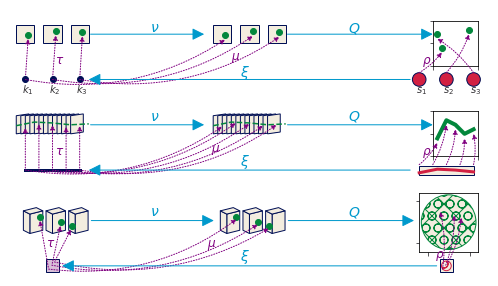
\includegraphics[width=\linewidth]{teaser.png}
  \caption{this is our model basically...}
  \label{fig:teaser}
}

%% Uncomment below to disable the manuscript note
%\renewcommand{\manuscriptnotetxt}{}

%% Copyright space is enabled by default as required by guidelines.
%% It is disabled by the 'review' option or via the following command:
% \nocopyrightspace


\vgtcinsertpkg

%%%%%%%%%%%%%%%%%%%%%%%%%%%%%%%%%%%%%%%%%%%%%%%%%%%%%%%%%%%%%%%%
%%%%%%%%%%%%%%%%%%%%%% START OF THE PAPER %%%%%%%%%%%%%%%%%%%%%%
%%%%%%%%%%%%%%%%%%%%%%%%%%%%%%%%%%%%%%%%%%%%%%%%%%%%%%%%%%%%%%%%%

\begin{document}

%% The ``\maketitle'' command must be the first command after the
%% ``\begin{document}'' command. It prepares and prints the title block.

%% the only exception to this rule is the \firstsection command
\firstsection{Introduction}
\maketitle
The aim of this work is to rearchitecture Matplotlib to take advantage of developments in software design, data structures, and visualization to improve consistency, reusability, and discoverability, so domain specific tool developers can build structure preserving visualization tools.

The contribution of this work is
\begin{description}
  \item[Topological] topology preserving relationship between data and graphic via continuous maps
  \item[Equivariant] property preservation from data component to visual representation as equivariant maps that carry a homomorphism of monoid actions
  \item[Artist] functional oriented visualization tool architecture built on the mathematical model to demonstrate the utility of the model
  \item [Model] prototype of the architecture built on Matplotlib's infrastructure to demonstrate the feasibility of the model
\end{description}

\section{Related Work}
Most information visualization tools are tuned to data continuity \cite{HeerSoftware2006,toryRethinkingVisualizationHighlevel2004}. For example, the relational database is core to libraries built on top of Grammar of Graphics\cite{wilkinsonGrammarGraphics2005}, including ggplot\cite{wickhamGgplot2ElegantGraphics2016a}, protovis\cite{bostockProtoviz2009} and D3 \cite{bostockDataDrivenDocuments2011}, vega\cite{satyanarayanDeclarativeInteractionDesign2014} and altair\cite{vanderplasAltairInteractiveStatistical2018}. Images underpin scientific visualization tools such as Napari\cite{nicholas_sofroniew_2021_4533308} and ImageJ\cite{schneiderNIHImageImageJ2012} and  the digital humanaties oriented ImagePlot\cite{studiesCulturevisImageplot2021} macro. Neither the table nor image model on its own supports all the data types a typical general purpose visualization library needs to support; instead libraries such as Matplotlib\cite{hunterMatplotlib2DGraphics2007} and Vtk\cite{hanwellVisualizationToolkitVTK2015, geveci2012vtk} explicitly carry around different data representations for all the different types of data they encode.  Where GoG and ImageJ type libraries have very consistent APIs for their visualization tools because the data structure is the same, the APIs for visualizations in VTK and Matplotlib are significantly dependent on the structure of the data it expects. This has lead to poor API consistency and brittle code as every visualization type has a very different point of view on how the data is structured. We present a model that has a single core data abstraction for the API consistency benefits, but the abstraction is general enough to provide a common interface for many different types of visualization.

The structure visualizations are expected to preserve is encoded in the connectivity of the records and in the properties of the variables in the dataset. Fiber bundles were proposed by Butler as one way to encode the continuity of the data separately from the types of variables \cite{butlerVisualizationModelBased1989,butlerVectorBundleClassesForm1992}. Our model builds on this work because the abstraction of data and flexible enough to support discrete and ND continuous datasets. Since Butler's model lacks a robust way of describing variables, we fold in Spivak's Simplicial formulation of databases \cite{spivakDatabasesAreCategories2010,spivakSIMPLICIALDATABASES} so that we can encode a schema like description of the data in the fiber bundle. One way of describing the binding between the schame and the continuinity is using the notion of structural \textit{keys} with associated \textit{values} proposed by Munzner\cite{munznerVisualizationAnalysisDesign2014}. Unlike Munzner's model where the semantic meaning of the key is tightly coupled to the position of the value in the dataset, our model considers keys to be a pure reference to topology. This allows the metadata to be altered, for example by changing the coordinate systems or time resolution, without imposing new semantics on the underlying structure. 
Visual representations of data, by definition, reflect something of the underlying structure and semantics\cite{friendlyBriefHistoryData2008}, whether through direct mappings from data into visual elements or via figurative representations that have meaning due to their similarity in shape to external concepts \cite{byrneAcquiredCodesMeaning2016}. The components of a visual representation were first codified by Bertin\cite{bertinSemiologyGraphicsDiagrams2011a}, and the notion that the properties of the data and visual representation match is the basis of most evaluations of visualization. Expressiveness, as defined by Mackinlay \cite{mackinlayAUTOMATICDESIGNGRAPHICAL1987, mackinlayAutomatingDesignGraphical1986} is a measure of how much of the structure any map can encode. A fully expressive component is one that is equivariant since it has preserved all the structure in the data. 

Models of visualization evaluate this equivariance and how elements built in the model can be composed to build more complex visualizations. Mackinlay's A Presentation Tool introduced the notion of visualizations having syntax and semantics \cite{mackinlayAutomatingDesignGraphical1986} and Wilkenson described the grammar of this language \cite{wilkinsonGrammarGraphics2005}. This grammar oriented approach allows users to describe how to compose visual elements into a graphical design \cite{wongsuphasawatNavigatingWideWorld2021}, while we are proposing a framework for building those elements. This same limitation is explicitly stated in the functional dependency notion of visualization developed by Sugibuchi\cite{sugibuchiFramwork2009} and evident in Vickers' category theory oriented framework in which semiotics are commutative. The algebraic process model by Kindlmann and Scheideggar proposes that the data and visualization transformations are commutative; while similar to our framework, it is missing any explicit mention of continuity. 

\section{Topological Equivariant Artist Model}
\label{sec:math}
We introduce the notion of an artist $\mathscr{\vartist}$ as an equivariant map from data to graphic
\begin{equation}
    \label{eq:artist}
    \mathscr{\vartist}: \mathscr{\dtotal} \rightarrow \mathscr{\gtotal}
\end{equation}
that carries a homomorphism of monoid actions $\varphi: \monoid \rightarrow \monoid^{\prime}$ \cite{cegarraCohomologyMonoidsOperators2019}, which are discussed in detail in section~\ref{sec:data_monoid}. Given \monoid\ on data $\mathscr{\dtotal}$ and $\monoid^{\prime}$ on graphic $\mathscr{\gtotal}$, we propose that artists $\mathscr{\vartist}$ are equivariant maps 
\begin{equation}
\mathscr{\vartist}(m\cdot \delement) = \varphi(m)\cdot\mathscr{\vartist}(\delement) 
\end{equation}
such that applying a monoid action $m \in \monoid$ to the data $\delement \in \mathscr{\dtotal}$ input to $\mathscr{\vartist}$ is equivalent to applying a monoid action $\varphi(\monoid) \in \monoid^{\prime}$ to the graphic $\vartist(\delement) \in \mathscr{\gtotal}$ output of the artist.
We model the data $\mathscr{\dtotal}$, graphic $\mathscr{\gtotal}$, and intermediate visual encoding $\mathscr{\vtotal}$ stages of visualization as topological structures that encapsulate types of variables and continuity; by doing so we can develop implementations that keep track of both in ways that let us distribute computation while still allowing assembly and dynamic update of the graphic. 
\subsection{Data Bundle}
\label{sec:math:data}
Building on Butler's proposal of using fiber bundles as a common data representation structure for visualization data\cite{butlerVectorBundleClassesForm1992, butlerVisualizationModelBased1989}, a fiber bundle is a tuple $(\dtotal,\,\dbase,\,\pi ,\,\dfiber)$ defined by the projection map $\pi$
\begin{equation}
    \label{eq:fiber_bundle}
    \begin{tikzcd}
        \dfiber \arrow[r, hook] & \dtotal \arrow[r, "\pi"] & \dbase
    \end{tikzcd}
\end{equation}
that binds the components of the data in \dfiber\ to the continuity represented in \dbase. By definition fiber bundles are locally trivial\cite{spanier1989algebraic,LocallyTrivialFibre}, meaning that over a localized neighborhood we can dispense with extra structure on \dtotal\ and focus on the components and continuity.

\subsubsection{Fiber Space: Variables}
\label{sec:math:data:fiber}
\begin{figure}[tb]
  \centering % avoid the use of \begin{center}...\end{center} and use \centering instead (more compact)
  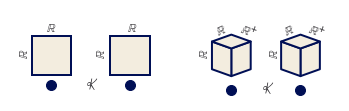
\includegraphics[width=\columnwidth]{fiber.png}
  \caption{These two datasets have the same base space \dbase\ of discrete points, but the square is a visual representation of the fiber space  $\dfiber=\reals\times\reals$, while the cube is a representation of $\dfiber=\reals\times\realsp\times\reals$}
  \label{fig:data_fiber}
\end{figure}

To formalize the structure of the data components, we use notation introduced by Spivak \cite{spivakSIMPLICIALDATABASES} that binds the components of the fiber to variable names. Spivak constructs a set \ftotal\ that is the disjoint union of all possible objects of types $\{\ftype_0, \ldots, \ftype_m\} \in \ftypes$, where \ftypes\ are the data types of the variables in the dataset. He then defines the single variable set \fttype\ 
\begin{equation}
    \label{eq:data_types}
    \begin{tikzcd}
        \fttype \arrow[r] \arrow[d, "\pi_{\fsection}"'] & \ftotal \arrow[d, "\pi"] \\
        \fnames \arrow[r, "\fsection"']                          & \ftypes       
    \end{tikzcd}
\end{equation}
which is \ftotal\ restricted to objects of type \ftype\ bound to variable name \fname. The \fttype\ lookup is by name to specify that every component is distinct, since multiple components can have the same type \ftype. Given \fsection, the fiber for a one variable dataset is
\begin{equation}
    \dfiber = \ftotal_{\fsection(\fname)} = \ftotal_{\ftype} 
\end{equation}
where \fsection\ is the schema binding variable name \fname\ to its datatype \ftype. A dataset with multiple variables has a fiber that is the cartesian cross product of $\ftotal_{\fsection}$ applied to all the columns:
\begin{equation}
F = \ftotal_{\fsection(\fname_{1})}\times \ldots \ftotal_{\fsection(\fname_{i})} \ldots\times \ftotal_{\fsection(\fname_{n})}
\end{equation}
which is equivalent to 
\begin{equation}
    \label{eq:math:data:fiber:decompose}
    \dfiber= \dfiber_{0} \times \ldots \times \dfiber_{i}\times\ldots\times \dfiber_{n}
\end{equation}
which allows us to decouple \dfiber\ into components $\dfiber_i$. Each component of \dfiber\ is a dimension of the topological fiber space, as illustrated in \autoref{fig:data_fiber}. The space $\dfiber=\reals\times\reals$ encodes that the dataset has two quantative continuous variables, while $\dfiber=\reals\times\reals\realsp$ encodes a dataset with three quantative contunous variables, one of which must be positive. 

\subsubsection{Equivariant Variable Properties: Monoid Actions}
\label{sec:math:data:monoid}
While structure on a set of values is often described algebraically as operations or through the actions of a group, for example Steven's measurement scales \cite{stevensTheoryScalesMeasurement1946, leaFormalizationMeasurementScale}, we generalize to monoids to support partial orderings. A partial ordering allows for multiple measurement values to have the same rank\cite{fongInvitationAppliedCategory2019}, which is useful for visualizing many types of multi indicator systems\cite{bruggemannRankingPrioritizationMultiindicator2011}. 

A monoid \cite{Monoid2021} $\monoid$ is a set with an associative binary operator $\ast:\monoid \times \monoid\rightarrow \monoid$. A monoid has an identity element $e\in \monoid$ such that $e\ast a= a \ast e = a$ for all $a \in \monoid$. As defined on a component of \dfiber, a left monoid action \cite{SemigroupAction2021,ActionNLab} of $\monoid_i$ is a set $\dfiber_i$ with an action $\bullet: \monoid\times \dfiber_i \rightarrow \dfiber_i$ with the properties:
\begin{align*}
    \textbf{associativity}\;& \text{for all } f,g \in \monoid_i \text{ and } x\in \dfiber_i,\, f\bullet(g\bullet x) = (f\ast g) \bullet x\\
    \textbf{identity}\;& \text{for all } x\in \dfiber_i, e\in \monoid_i,\,  e\bullet x = x 
\end{align*}
As with the fiber \dfiber\, the total monoid space \monoid\ is the cartesian product
\begin{equation}
\monoid= \monoid_{0} \times \ldots \times \monoid_{i}\times \ldots \times\ldots \monoid_{n}
\end{equation}
of each monoid $\monoid_{i}$ on $\dfiber_{i}$.  The monoid is also added to the specification of the fiber $(\fname_i,\, \ftype_i,\, \fttype\, \monoid_i)$

Defining the monoid actions on the components serves as the basis for identifying the invariance\cite{kindlmannAlgebraicProcessVisualization2014} that must be preserved in the visual representation of the component. A secondary advantage of defining structure in terms of monoids is that they are commonly found in functional programming because they specify compositions of transformations \cite{yorgeyMonoidsThemeVariations, stievenMonadJustMonoid2020}.

\subsubsection{Base Space: Continuity}
\label{sec:math:data:base}
 The base space \dbase\ is way to express how the records in \dtotal\ are connected to each other, for example if they are discrete points or if they lie in a 2D continous surface. Formally \dbase\ is the quotient space of \dtotal\, meaning it is the finest space\cite{aurouxMath131Introduction} such that every $\dbasepoint \in \dbase$ has a corresponding fiber $\dfiber_k$\cite{QuotientSpaceTopology2020}. Our model formulates \dbase\ as akin to an indexing space into \dtotal\ that describes the structure of \dtotal.  
 
 \begin{figure}[tb]
  \centering % avoid the use of \begin{center}...\end{center} and use \centering instead (more compact)
  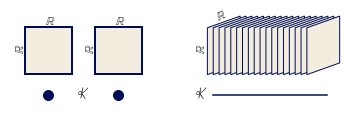
\includegraphics[width=\columnwidth]{base.png}
  \caption{These two datasets have the same fiber space  $\dfiber=\reals\times\reals$, but the left dataset has a discrete continuity while the right is 1D continuous over the interval $\left[0,1\right]$.}
  \label{fig:data_continuity}
 \end{figure}

 As illustrated in ~\autoref{fig:data_continuity}, \dbase\ can have any number of dimensions, can be continuous or discrete, and is somewhat independent of the dimensions of the fiber. As with fibers and monoids, we can decompose the total space into components $\pi:\dtotal_i\rightarrow \dbase$ where
 \begin{equation}
    \label{eq:math:data:base:decompose}
     \pi:\dtotal_1\oplus\ldots\oplus \dtotal_i \oplus\ldots \oplus \dtotal_n \rightarrow \dbase
 \end{equation}
 which is a decomposition of \dfiber. The \dbase\ remains the same because the connectivity of records does not change just because there are fewer elements in each record. By encoding this continuity in the model as \dbase\, the data model now explicitly carries information about its structure such that the implicit assumptions of the visualization algorithms are now explicit. The explicit topology is a concise way of distinguishing visualizations that appear identical, for example heatmaps and images.  

 \subsubsection{Section: Values}
 \label{sec:math:data:section}
 \begin{figure}[tb]
  \centering % avoid the use of \begin{center}...\end{center} and use \centering instead (more compact)
  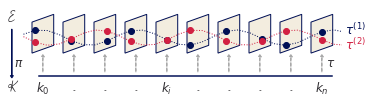
\includegraphics[width=\columnwidth]{fiberbundle.png}
  \caption{Each section in the fiber bundle is a unique continuous map from base space to fiber encoding the set of records in the dataset. The two sections, $\dsection^{(1)}$ and $\dsection^{(2)}$, shown here are in the set of global sections $\Gamma(\dtotal)$.}
  \label{fig:data_section}
 \end{figure}

 While the projection function $\pi:\dtotal \rightarrow\dbase$ ties together the base space \dbase\ with the fiber \dfiber, a section $\dsection: \dbase\rightarrow \dtotal$ encodes a dataset. A section function takes as input location $\dbasepoint \in \dbase$ and returns a record $\delement \in \dtotal$. For any fiber bundle, there exists a map
 \begin{equation}
     \begin{tikzcd}
         \dfiber \arrow[r, hook] & \dtotal \arrow[d, "\pi"'] \\
                           & \dbase \arrow[u, "\dsection"', bend right]
     \end{tikzcd}
 \end{equation}
  such that $\pi(\dsection(\dbasepoint)) = \dbasepoint$. The set of all global sections is denoted as $\Gamma(\dtotal)$. As illustrated in \autoref{fig:data_section}, the section is a continuous mapping from a location $\dbasepoint \in \dbase$ on the base space to a record $\delement \in \dfiber$ in the fiber. Assuming a trivial fiber bundle $\dtotal = \dbase \times \dfiber$, the section is 
 \begin{equation}
     \label{eq:section_return}
     \dsection(\dbasepoint) = (\dbasepoint, (g_{\dfiber_{0}}(\dbasepoint), \ldots, g_{\dfiber_{n}}(\dbasepoint)))
 \end{equation}
 where $g: \dbase \rightarrow \dfiber$ is the index function into the fiber component. This formulation of the section also holds on locally trivial sections of a non-trivial fiber bundle. As with \autoref{eq:math:data:fiber:decompose} and \autoref{eq:math:data:base:decompose}, \dsection\ can be decomposed into components 
 \begin{equation}
 \label{eq:math:data:section:decompose}
 \dsection= (\dsection_0,\ldots, \dsection_i, \dots, \dsection_n) 
 \end{equation}
 where each section $\dsection_i$ maps into a record on a component $\dfiber_i \in \dfiber$. This allows for accessing the data component wise in addition to accessing the data in terms of its location over \dbase.

 \subsubsection{Sheafs: Gluing Sections }
 The restriction maps of a sheaf describe how local sections $\iota^{*}\dsection$ over a neighborhood $U$ around \dbasepoint\ can be glued into larger sections \cite{ghristElementaryAppliedTopology2014,ghristHomologicalAlgebraData2018}. This puts a continuous structure on local sections, which allows for defining a section over a subset in \dbase. The inclusion map $\iota: U \rightarrow \dbase$ pulls \dtotal\ over $U$ 
 \begin{equation}
     \label{eq:sheaf}
     \begin{tikzcd}
         \iota^*\dtotal \arrow[d, "\pi"'] \arrow[r, "\iota^*", hook]             & \dtotal \arrow[d, "\pi"']                  \\
         U \arrow[r, "\iota", hook] \arrow[u, "\iota^{*}\dsection"', bend right] & \dbase \arrow[u, "\dsection"', bend right]
     \end{tikzcd}
 \end{equation}
 such that the pulled back $\iota^*\dsection$ only contains records over $U \subset \dbase$. Gluing together $\iota^*\dsection$ sections is necessary for navigation techniques such as pan and zoom\cite{NekrasovskiEvaluationPanZoom2006} and dynamically updated visualizations such as sliding windows\cite{crouchDynamicGraphsSlidingwindow2013,chuTimeSeriesSegmentation1995}. 

 \subsection{Graphic Bundle}
 \label{sec:math:graphic}  
We introduce a graphic bundle to hold the essential information necessary to render a graphical design constructed by the artist. As with the data, we can represent the target graphic as a section \gsection\ of a bundle  $(\gtotal, \gbase, \pi, \gfiber)$
\begin{equation}
  \begin{tikzcd}[ampersand replacement=\&]
      \gfiber \arrow[r, hook] \& \gtotal \arrow[d, "\pi"'] \\
                        \& \gbase \arrow[u, "\gsection"', bend right]
  \end{tikzcd}
\end{equation}
where \gsection\ is the fully encoded graphic. To fully specify the visual characteristics of the image, we construct a fiber \gfiber\ that is an infinite resolution version of the target space. Typically \gtotal\ is trivial and therefore sections can be thought of as mappings into \gfiber. In this work, we assume a 2D opaque image $\gfiber=\reals^5$ with elements 
\begin{equation}
(x,\, y,\, r,\, g,\, b) \in \gfiber
\end{equation}
such that a rendered graphic only consists of 2D position and color. By abstracting the target display space as \gfiber, the model can support different targets, such as a 2D screen or 3D printer. 

\subsubsection{Equivariant Topology: Graphic Base Space}
\label{sec:math:graphic:base}
\begin{figure}[tb]
  \centering % avoid the use of \begin{center}...\end{center} and use \centering instead (more compact)
  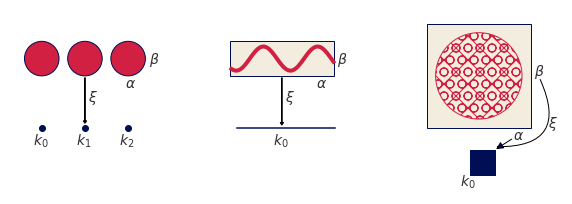
\includegraphics[width=\columnwidth]{retraction_maps.png}
  \caption{The 0D scatter \dbasepoint\ and 1D line \dbasepoint\ are thickened into \gbase\ with coordinates $\gbasepoint=(\gx, \gy)$ that are a region in an idealized 2D screen. The image has the same dimension in \gbase\ as in \dbase.}
  \label{fig:graphic_base}
 \end{figure}

Just as the \dbase\ encodes the connectivity of the records in the data, we propose an equivalent \gbase\ that encodes the connectivity of the rendered elements of the graphic. Formally, we require that \dbase\ be a deformation retract\cite{RetractionTopology2020} of \gbase\ so that \dbase\ and \gbase\ have the same homotopy. The surjective map $\vindex: \gbase \rightarrow \dbase$ 
\begin{equation}
    \begin{tikzcd}
        \dtotal \arrow[d, "\pi"'] & \gtotal \arrow[d, "\pi"'] \\
        \dbase                   & \gbase \arrow[l, "\vindex"']
    \end{tikzcd}
\end{equation}
goes from region $\gbasepoint \in \gbase_{\dbasepoint}$ to its associated point $\gbasepoint$. While \gbase\ must have the same continuity as \dbase\, it is sometimes the  thickened version shown in \autoref{fig:graphic_base}. This thickening is necessary when the dimensionality of \dbase\ is less than the dimensionality of the target display. For example, a \dbasepoint\ that is 0D in \dbase\ cannot be represented on screen unless it is thickened to 2D to encode the connectivity of the points in \gfiber\ that visually represent the record at \dbasepoint. 

\subsection{Artist}
The topological artist \vartist\ is a monoid equivariant sheaf map from the sheaf on a data bundle \dtotal\ which is $\mathcal{O}(\dtotal)$ to the sheaf on the graphic bundle \gtotal, $\mathcal{O}(\gtotal)$. 
\begin{equation}
    \vartist: \mathcal{O}(\dtotal) \rightarrow \mathcal{O}(\gtotal)
\end{equation}
While \vartist\ can usually construct graphical elements solely with the data in \dsection, some visualizations, such as line, may also need some finite number $n$ of derivatives, which is captured by the jet bundle $\mathcal{J}^n$ \cite{JetBundle2020,musilovaCalculusVariationsJet2016} with $\mathcal{J}^{0}(\dtotal)=\dtotal$. In this work, we at most need $\mathcal{J}^{2}(\dtotal)$ which is the value at \dsection\ and its first and second derivatives; therefore the artist takes as input the jet bundle $\dtotal^{\prime}=\mathcal{J}^{2}(\dtotal)$. 

Specifically, \vartist is the equivariant map from $\dtotal^{\prime}$ to a specific graphic $\gsection \in \Gamma(H)$ 
\begin{equation}
    \label{eq:math:artist:diagram}
    \begin{tikzcd}
        \dtotal^{\prime} \arrow[r, "\vchannel"] \arrow[rd, "\pi"'] & \vtotal \arrow[d, "\pi"] & \vindex^*\vtotal \arrow[r, "\vmark"] \arrow[d, "\vindex^*\pi"'] \arrow[l, "\vindex^*"'] & \gtotal \arrow[ld, "\pi"] \\
                                              & \dbase                  & \gbase \arrow[l, "\vindex"']                                              &                    
        \end{tikzcd}
\end{equation}
where the input can be point wise $\dsection(\dbasepoint)\mid \dbasepoint \in \dbase$. The visual bundle $(\vtotal,\,\dbase,\,\pi ,\,\vfiber)$ is the latent space of possible parameters of a visualization type, such as a scatter or line plot. As with the data and graphic bundles, the visual bundle is  defined by the projection map $\pi$
\begin{equation}
    \begin{tikzcd}[ampersand replacement=\&]
        \vfiber \arrow[r, hook] \& \vtotal \arrow[d, "\pi"'] \\
                          \& \dbase \arrow[u, "\vsection"', bend right]
    \end{tikzcd}
\end{equation}
where \vsection\ is the visual variable encoding\cite{bertinSemiologyGraphicsDiagrams2011a} of the data section \dsection. The visual fiber \vfiber\ is defined in terms of the input parameters of the visualization library's plotting functions; by making these parameters explicit components of the fiber, we can build consistent definitions and expectations of how these parameters behave. 

In \autoref{eq:math:artist:diagram}, the encoders $\vchannel:\dtotal^{\prime} \rightarrow \vtotal$ convert the data components to visual components. The continuity map $\vindex:\gbase \rightarrow \dbase$ then pulls back the visual bundle \vtotal\ over \gbase. Then the assembly function $\vmark: \vtotalpull \rightarrow \gtotal$ composites the fiber components of \vtotalpull\ into a graphic in \gtotal. This functional decomposition of the visualization artist facilitates building reusable components at each stage of the transformation because the equivariance constraints are defined on \vchannel, \vmark, and \vindex. We name this map the artist as that is the analogous part of the  Matplotlib\cite{hunterArchitectureOpenSource} architecture that builds visual elements.

\section{Prototype}



\subsubsection{Ejector Seat Reservation}

Duis autem~\cite{Lorensen:1987:MCA}\footnote{The algorithm behind
Marching Cubes \cite{Lorensen:1987:MCA} had already been
described by Wyvill et al. \cite{Wyvill:1986:DSS} a year
earlier.} vel eum iriure dolor in hendrerit
in vulputate velit esse molestie consequat,\footnote{Footnotes
appear at the bottom of the column.} vel illum dolore eu
feugiat nulla facilisis at vero eros et accumsan et iusto odio
dignissim qui blandit praesent luptatum zzril delenit augue duis
dolore te feugait nulla facilisi. Lorem ipsum dolor sit amet,
consectetuer adipiscing elit, sed diam nonummy nibh euismod tincidunt
ut laoreet dolore magna aliquam erat volutpat.


\paragraph{Confirmed Ejector Seat Reservation}

Ut wisi enim ad minim veniam, quis nostrud exerci tation ullamcorper
suscipit lobortis nisl ut aliquip ex ea commodo
consequat~\cite{Nielson:1991:TAD}. Duis autem vel eum iriure dolor in
hendrerit in vulputate velit esse molestie consequat, vel illum dolore
eu feugiat nulla facilisis at vero eros et accumsan et iusto odio
dignissim qui blandit praesent luptatum zzril delenit augue duis
dolore te feugait nulla facilisi.

\paragraph{Rejected Ejector Seat Reservation}

Ut wisi enim ad minim veniam, quis nostrud exerci tation ullamcorper
suscipit lobortis nisl ut aliquip ex ea commodo consequat. Duis autem
vel eum iriure dolor in hendrerit in vulputate velit esse molestie

\subsection{Vestibulum}

Vestibulum ut est libero. Suspendisse non libero id massa congue egestas nec at ligula. Donec nibh lorem, ornare et odio eu, cursus accumsan felis. Pellentesque habitant morbi tristique senectus et netus et malesuada fames ac turpis egestas. Donec dapibus quam vel eros mattis, id ornare dolor convallis. Donec at nisl sapien. Integer fringilla laoreet tempor. Fusce accumsan ante vel augue euismod, sit amet maximus turpis mattis. Nam accumsan vestibulum rhoncus. Aenean quis pellentesque augue. Suspendisse sed augue et velit consequat bibendum id nec est. Quisque erat purus, ullamcorper ut ex vel, dapibus dignissim erat.

Quisque sit amet orci quam. Lorem ipsum dolor sit amet, consectetur adipiscing elit. Aliquam pharetra, nunc non efficitur convallis, tellus purus iaculis lorem, nec ultricies dolor ligula in metus. Class aptent taciti sociosqu ad litora torquent per conubia nostra, per inceptos himenaeos. Aenean eu ex nulla. Morbi id ex interdum, scelerisque lorem nec, iaculis dui. Phasellus ultricies nunc vitae quam fringilla laoreet. Quisque sed dolor at sem vestibulum fringilla nec ac augue. Ut consequat, velit ac mattis ornare, eros arcu pellentesque erat, non ultricies libero metus nec mi. Sed eget elit sed quam malesuada viverra. Quisque ullamcorper, felis ut convallis fermentum, purus ligula varius ligula, sit amet tempor neque dui non neque. Donec vulputate ultricies tortor in mollis.

Integer sit amet dolor sit amet turpis ullamcorper varius. Cras volutpat bibendum scelerisque. Maecenas mauris dolor, gravida eu elit et, sodales consequat tortor. Integer id commodo elit. Pellentesque sollicitudin ex non nulla molestie eleifend. Mauris sagittis metus nec turpis imperdiet, vel ullamcorper nibh tincidunt. Sed semper tempus ex, ut aliquet erat hendrerit id. Maecenas sit amet dolor sollicitudin, luctus nunc sit amet, malesuada justo.

Mauris ut sapien non ipsum imperdiet sodales sit amet ac diam. Nulla vel convallis est. Etiam dapibus augue urna. Aenean enim leo, fermentum quis pulvinar at, ultrices quis enim. Sed placerat porta libero et feugiat. Phasellus ullamcorper, felis id porta sollicitudin, dolor dui venenatis augue, vel fringilla risus massa non risus. Maecenas ut nulla vitae ligula pharetra feugiat non eu ante. Donec quis neque quis lorem cursus pretium ac vulputate quam. Cras viverra tellus vitae sapien pretium laoreet. Pellentesque fringilla odio venenatis ex viverra, quis eleifend tortor ornare. Ut ut enim nunc. Vivamus id ligula nec est dignissim eleifend.

Nunc ac velit tellus. Donec et venenatis mauris. Lorem ipsum dolor sit amet, consectetur adipiscing elit. Ut vitae lectus vel ante mollis congue. Vestibulum at cursus velit. Curabitur in facilisis enim. Vestibulum eget dui aliquet risus laoreet laoreet. Phasellus et est id magna interdum venenatis. Donec luctus vehicula justo sed laoreet. Quisque tincidunt suscipit augue, in molestie sem accumsan sed.
\section{Conclusion}

Lorem ipsum dolor sit amet, consetetur sadipscing elitr, sed diam
nonumy eirmod tempor invidunt ut labore et dolore magna aliquyam erat,
sed diam voluptua. At vero eos et accusam et justo duo dolores et ea
rebum. Stet clita kasd gubergren, no sea takimata sanctus est Lorem
ipsum dolor sit amet. Lorem ipsum dolor sit amet, consetetur
sadipscing elitr, sed diam nonumy eirmod tempor invidunt ut labore et
dolore magna aliquyam erat, sed diam voluptua. At vero eos et accusam
et justo duo dolores et ea rebum. Stet clita kasd gubergren, no sea
takimata sanctus est Lorem ipsum dolor sit amet. Lorem ipsum dolor sit
amet, consetetur sadipscing elitr, sed diam nonumy eirmod tempor
invidunt ut labore et dolore magna aliquyam erat, sed diam
voluptua. At vero eos et accusam et justo duo dolores et ea
rebum.


%% if specified like this the section will be committed in review mode
\acknowledgments{
The authors wish to thank A, B, and C. This work was supported in part by
a grant from Chan Zuckerberg Institute  (\# 12345-67890).}

%\bibliographystyle{abbrv}
\bibliographystyle{abbrv-doi}
%\bibliographystyle{abbrv-doi-narrow}
%\bibliographystyle{abbrv-doi-hyperref}
%\bibliographystyle{abbrv-doi-hyperref-narrow}
\bibliography{../draft/glasslab_viz.bib}

\end{document}

